\documentclass[tikz, border=10pt]{standalone}
\tikzset{
    vertex/.style = {
        circle,
        fill            = black,
        outer sep = 2pt,
        inner sep = 1pt,
    }
}
\usepackage{xcolor}
\begin{document}
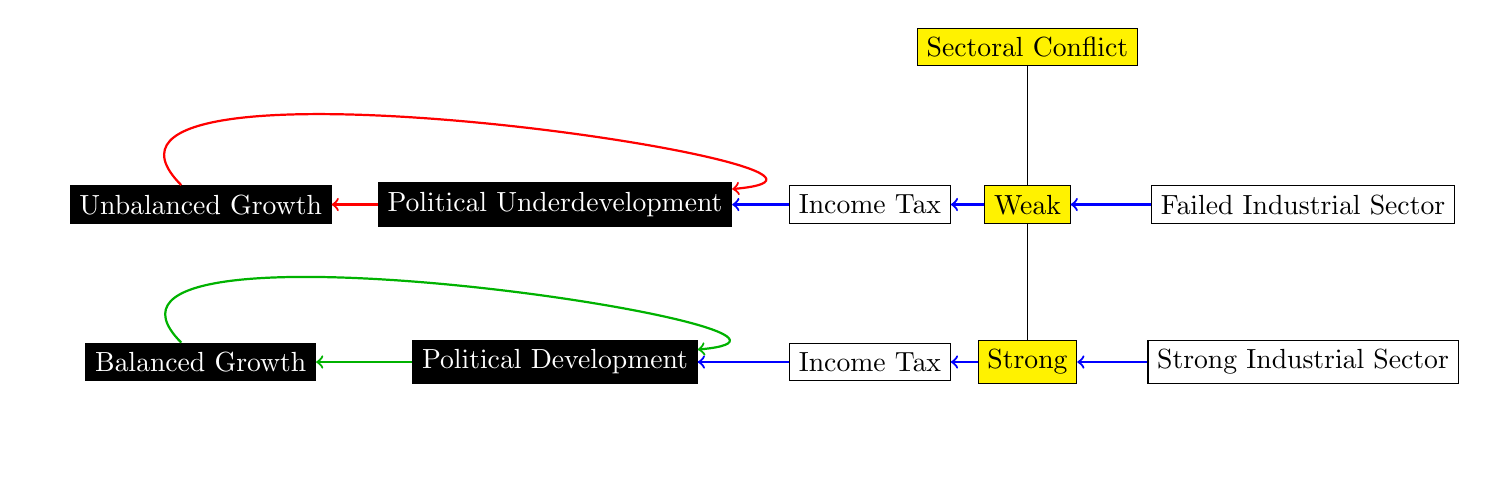
\begin{tikzpicture}
    
  % Opposition
  \node[draw,fill=black,text=white] (ArgumentA) at (1,0) {Balanced Growth};
  \node[draw,fill=black,text=white] (ArgumentB) at (5.5,0) {Political Development};
  \node[draw] (ArgumentC) at (9.5,0) {Income Tax};
  \node[draw,fill=yellow,text=black] (ArgumentD2) at (11.5,0) {Strong};
  \node[draw] (ArgumentE) at (15,0) {Strong Industrial Sector};




\draw[<-,draw=blue,thick] (ArgumentB) to (ArgumentC);
\draw[->,draw=black!30!green,thick] (ArgumentB) to (ArgumentA);
\draw[<-,draw=black!30!green,thick] (ArgumentB) to[out=5] (ArgumentA);
\draw[->,draw=blue,thick] (ArgumentD2) to (ArgumentC);
\draw[<-,draw=blue,thick] (ArgumentD2) to (ArgumentE);



  \node at (6., -1.0) {};


  % Opposition
  \node[draw,fill=black,text=white] (ArgumentA) at (1,2) {Unbalanced Growth};
  \node[draw,fill=black,text=white] (ArgumentB) at (5.5,2) {Political Underdevelopment};
  \node[draw] (ArgumentC) at (9.5,2) {Income Tax};
  \node[draw,fill=yellow,text=black] (ArgumentD) at (11.5,2) {Weak};
  \node[draw] (ArgumentE) at (15,2) {Failed Industrial Sector};
  \draw[<-,draw=blue,thick] (ArgumentD) to (ArgumentE);


  \node[draw,fill=yellow] (conflict) at (11.5,4) {Sectoral Conflict};
  \draw[-,draw=black] (conflict) to (ArgumentD);
  \draw[-,draw=black] (ArgumentD) to (ArgumentD2);


\draw[<-,draw=blue,thick] (ArgumentB) to (ArgumentC);
\draw[->,draw=red,thick] (ArgumentB) to (ArgumentA);
\draw[<-,draw=red,thick] (ArgumentB) to[out=5] (ArgumentA);
\draw[->,draw=blue,thick] (ArgumentD) to (ArgumentC);



  \node at (6., -1.0) {};
  
\end{tikzpicture}
\end{document}